Once the local SimCenter working environment has been tested and is
functioning correctly, the \texttt{\getsoftwarename{}} Application
can be tested. The simplest way to do this is by running an analysis
using the default structural model with synthetic wind event. By
doing this, it is not necessary to enter any information on the
structural model and only inputs for the synthetic wind forces 
and uncertainty quantification are required. With this quick setup, the
functionality of the \texttt{\getsoftwarename{}} UI and the associated backend
workflow can be tested. The necessary steps to perform this
testing are provided below.

A full description of how to use this software is provided
in \Cref{chap:usage}.  In this quick test, users will only
interface with the event tab (\texttt{EVT}), the uncertainty
quantification tab (\texttt{UQ}), and the results tab (\texttt{RES}).

The first step is to start the \texttt{\getsoftwarename{}}
application.  Once the application is started, the second step is to
input the parameters for the synthetic motions under the \texttt{EVT}
(Event) tab. This is shown in \Cref{fig:input_event}. Click
on the \texttt{EVT} tab which will allow the loading type to be
selected. From the dropdown menu select \texttt{Stochastic Wind Event}
model will be set as \texttt{Wittag and Sinha (1975)}.

\begin{figure}[!htbp]
  \centering {
    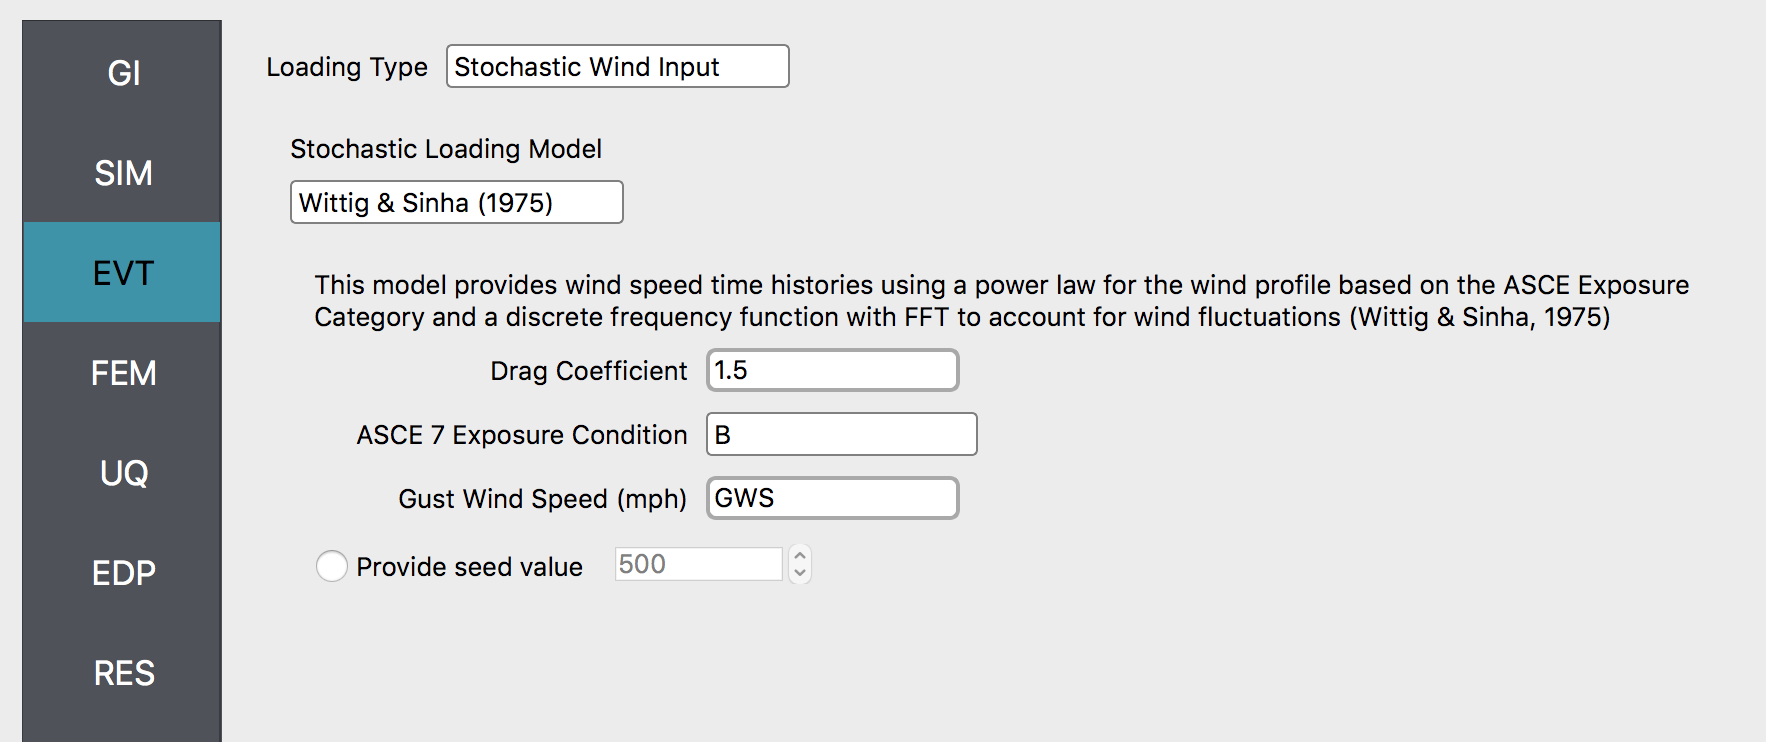
\includegraphics[width=0.7\textwidth]
    {installation/figures/testWE_EVT.png} }
  \caption{Selecting event type and inputting synthetic motion parameters}
  \label{fig:input_event}
\end{figure}

Only three inputs are required for this test, of which one will be set
to a random variable. As shown in \Cref{fig:input_event}, set the
\emph{Drag Coefficient} to {\texttt 1.5}, \emph{exposure condition} to \texttt{B}, and \emph{Gust Wind Speed} to \texttt{GWS}.
to \texttt{vs30}. The \texttt{Provide seed value} radio button should
be left unselected. By specifying these inputs, both drag coefficient
and the exposure condition will have constant values in all
realizations while \texttt{GWS} will have different values based on
the model parameters specified in the uncertainty quantification
(\texttt{UQ}) tab. With these inputs specified, navigate to
the \texttt{UQ} tab. Here the distributions and their relevant
parameters will be specified for the random variables defined in the
analysis\textemdash only $GWS$ in this case. Since $GWS$ was
identified as a random variable by inputting the parameter value as
text, it is automatically added as a random variable, as shown
in \Cref{fig:input_uq}. Set the distribution type to \texttt{normal}
with a \texttt{Mean} and \texttt{Standard Dev} of 100 and 10 mph,
respectively.

\begin{figure}[!htbp]
  \centering {
    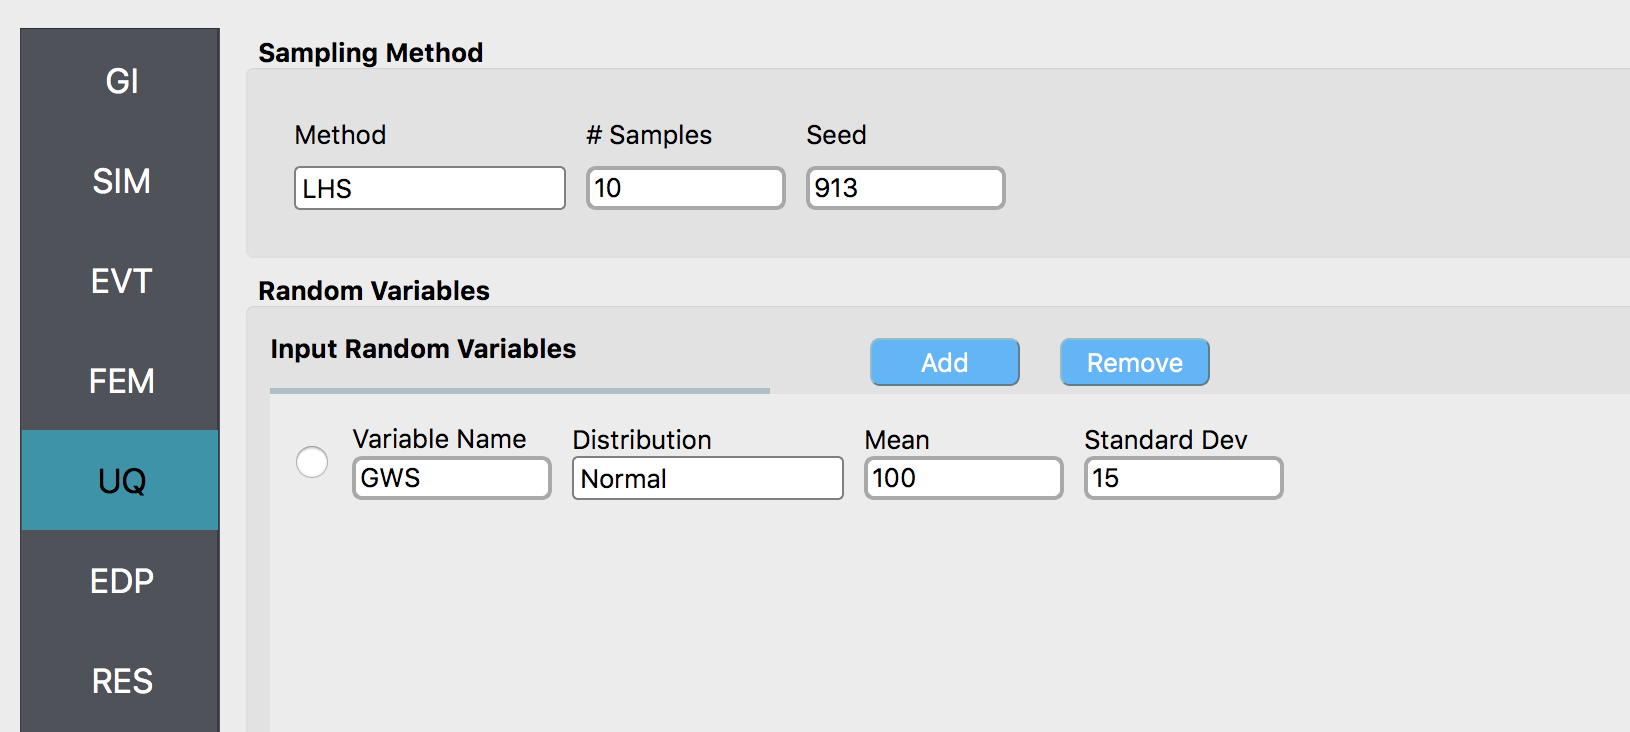
\includegraphics[width=0.7\textwidth]
    {installation/figures/testWE_UQ.png} }
  \caption{Specifying distribution type and parameters for random
  variables in analysis\textemdash only $GWS$ in this case}
  \label{fig:input_uq}
\end{figure}


Now, click on the \texttt{RUN} button, which will bring up a pop-up
menu that provides information on the application directory and
the working directory. The application directory should already be
automatically set to where \texttt{\getsoftwarename{}} is installed.
If desired, the working directory can be changed. In order to start
the analysis, click on the \texttt{Submit} button.

\begin{figure}[!htbp]
  \centering {
    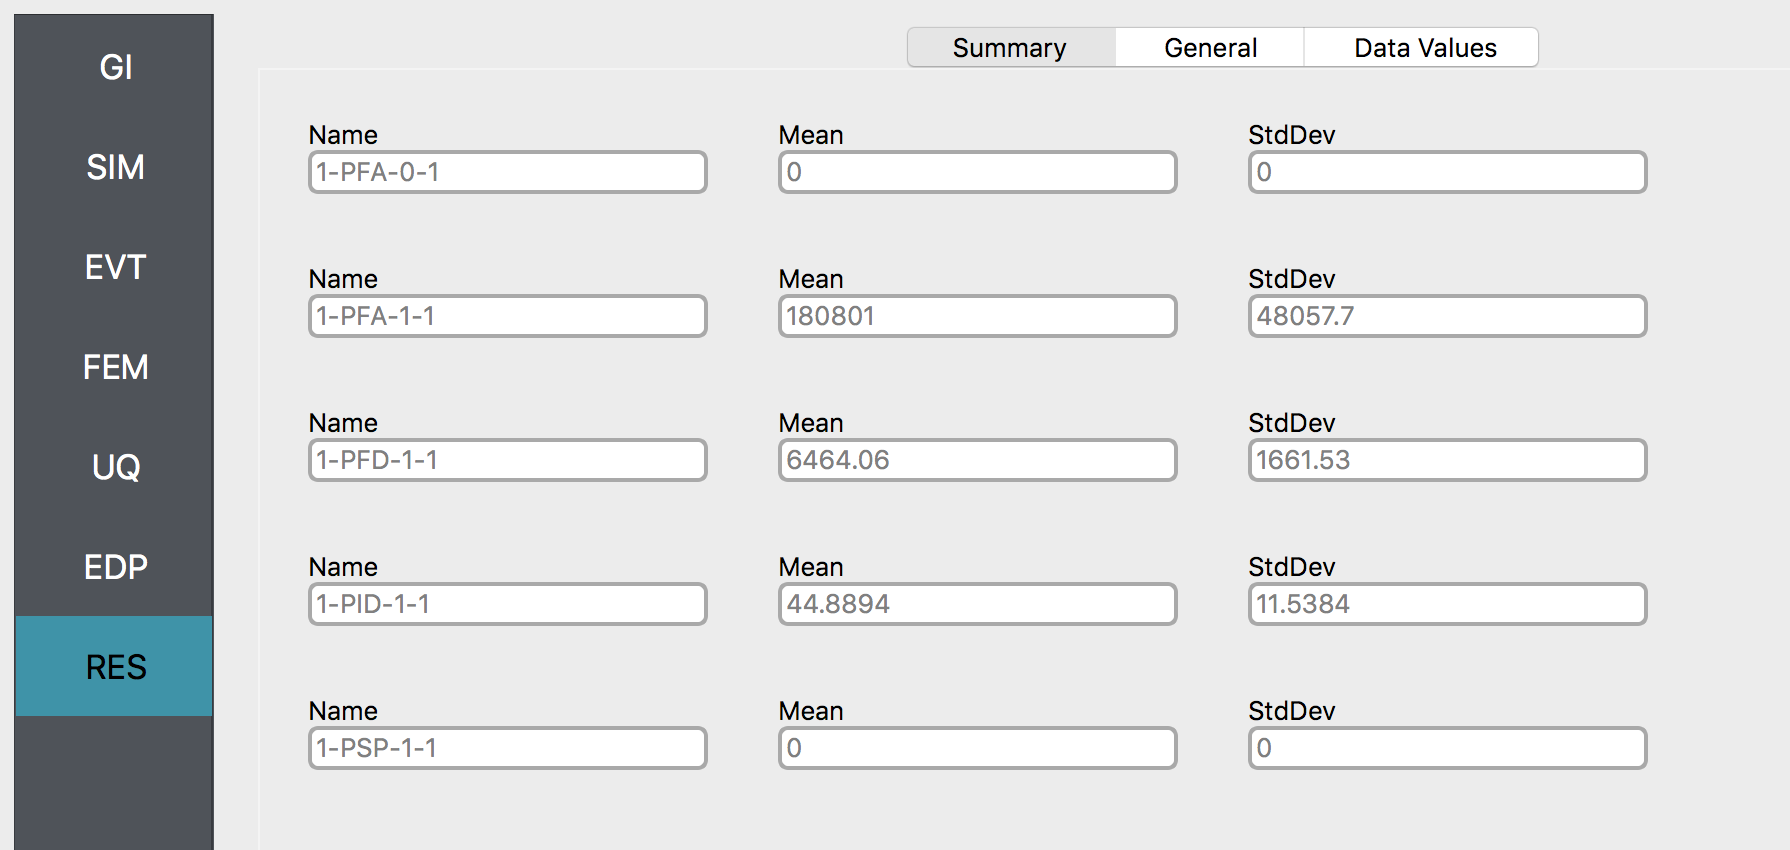
\includegraphics[width=0.7\textwidth]
    {installation/figures/testWE_RES.png} }
  \caption{Results for test analysis. This tab will open automatically
  when the analysis completes, indicating a successful installation}
  \label{fig:show_results}
\end{figure}



If successful, the application will pause briefly while it runs the
analysis before automatically displaying the simulations results in
the \texttt{RES} tab, as shown
in \Cref{fig:show_results}. Remember, the results shown
in \Cref{fig:show_results} most likely will not be the same as
those from this local test since $GWS$ is a random variable and
the values realized in the simulations will be different while still
following the same distribution. In any case, if the simulations
completed and the \texttt{RES} tab is showing simulation results, then
the \texttt{\getsoftwarename{}} App is properly installed and configured.
